%%%%%%%% ICML 2026 submission: frozen TSFMs for guided-wave SHM %%%%%%%%
\documentclass{article}

\usepackage{microtype}
\usepackage{graphicx}
\usepackage{subcaption}
\usepackage{booktabs}
\usepackage{array}
\usepackage{float}
\usepackage{hyperref}
\newcommand{\theHalgorithm}{\arabic{algorithm}}

% Blind submission (default). For a preprint with author names use
%   \usepackage[preprint]{icml2026}
% and for the camera-ready version use
%   \usepackage[accepted]{icml2026}
\usepackage{icml2026}

\usepackage{amsmath}
\usepackage{amssymb}
\usepackage{mathtools}
\usepackage[capitalize,noabbrev]{cleveref}
\usepackage{tikz}
\usetikzlibrary{arrows.meta,positioning,calc,shapes.geometric}

\definecolor{tsfmblue}{HTML}{2A78D6}
\definecolor{tsfmblue1}{HTML}{CDE2FB}
\definecolor{tsfmblue2}{HTML}{6DA7EC}
\definecolor{tsfmblue3}{HTML}{184F95}
\definecolor{dmgorange}{HTML}{EB6834}
\definecolor{inkgray}{HTML}{52514E}
\definecolor{rulegray}{HTML}{D9D8D3}

\newcommand{\fft}{$|$FFT$|$}
% primitive \input, so generated table rows can sit inside tabular
\makeatletter\newcommand{\inputrows}[1]{\@@input #1 }\makeatother

\icmltitlerunning{Frozen Time Series Foundation Models for Guided-Wave Structural Health Monitoring}

\begin{document}

\twocolumn[
  \icmltitle{Compare Like with Like: Frozen Time Series Foundation Models\\
    for Guided-Wave Structural Health Monitoring}

  % Author information is hidden automatically in the blind version.
  % TODO before a preprint or camera-ready: complete affiliation and e-mail.
  \begin{icmlauthorlist}
    \icmlauthor{Mahindra Rautela}{aff}
  \end{icmlauthorlist}
  \icmlaffiliation{aff}{Affiliation, City, Country}
  \icmlcorrespondingauthor{Mahindra Rautela}{email@example.com}

  \icmlkeywords{time series foundation models, structural health monitoring, guided waves,
    anomaly detection, damage localisation, transfer learning}

  \vskip 0.3in
]

\printAffiliationsAndNotice{}

\begin{abstract}
Time series foundation models (TSFMs) are pretrained on large and varied corpora, but it is not clear
whether their representations help with ultrasonic guided waves, the signals used to monitor composite
aircraft structures for damage. We test six frozen TSFMs as feature extractors on three public datasets
that cover the main monitoring tasks: supervised damage classification, unsupervised delamination
detection and damage localisation. The embeddings are useful when they are used the way engineers use
baseline measurements, by comparing each signal with healthy recordings from the same sensor path and
reading the sensor network as a whole. Used this way, frozen embeddings classify damage on held-out sensor
configurations with AUC up to 0.86, match classical baseline subtraction for delamination detection while
transferring better across specimens, and place all 28 held-out damage positions in the correct zone,
where a physics-based damage index reaches 0.89. Used one signal at a time, the same embeddings, like
every other method we tried, locate damage barely above chance. We also show how repeated acquisitions,
sign-inverted signals and baseline normalisation can inflate results on these datasets.
\end{abstract}

\begin{figure*}[t]
  \centering
  \resizebox{\textwidth}{!}{%
  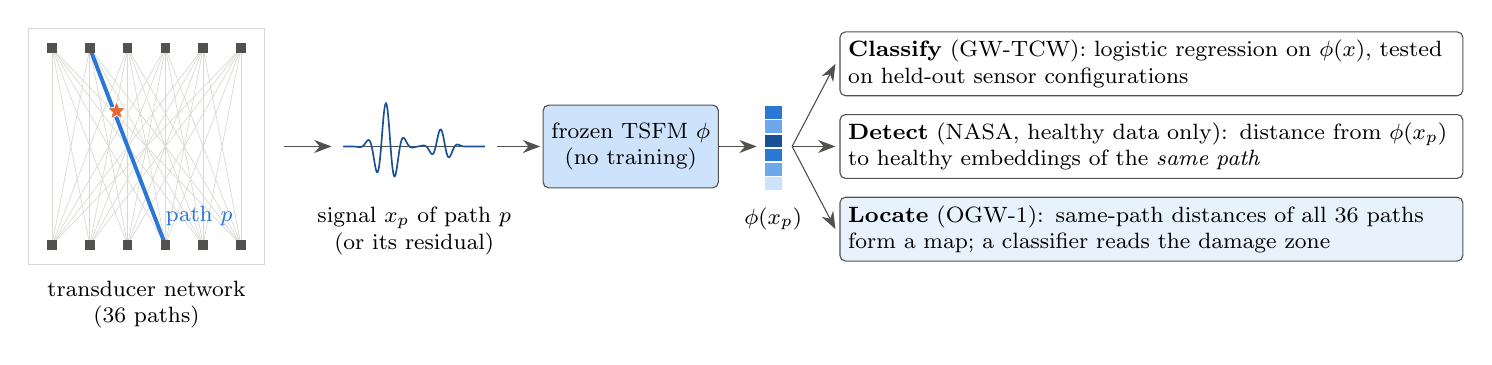
\begin{tikzpicture}[font=\footnotesize, >={Stealth[length=2.2mm]},
      box/.style={draw=inkgray, rounded corners=2pt, line width=0.4pt, align=left, inner sep=3pt}]
    % plate with transducer network
    \draw[rulegray, line width=0.5pt] (0,0) rectangle (3,3);
    \foreach \i in {0,...,5} {\foreach \j in {0,...,5} {
      \draw[rulegray, line width=0.25pt] (0.3+0.48*\i,2.75) -- (0.3+0.48*\j,0.25);}}
    \draw[tsfmblue, line width=1.4pt] (0.78,2.75) -- (1.74,0.25);
    \foreach \i in {0,...,5} {\fill[inkgray] (0.3+0.48*\i-0.06,2.69) rectangle ++(0.12,0.12);
                              \fill[inkgray] (0.3+0.48*\i-0.06,0.19) rectangle ++(0.12,0.12);}
    \node[star, star points=5, star point ratio=2.2, fill=dmgorange, draw=white, line width=0.3pt,
          minimum size=7pt, inner sep=0pt] at (1.12,1.95) {};
    \node[tsfmblue, anchor=west] at (1.62,0.62) {path $p$};
    \node[align=center, anchor=north] at (1.5,-0.08) {transducer network\\(36 paths)};
    % signal
    \draw[->, inkgray] (3.25,1.5) -- (3.85,1.5);
    \draw[inkgray, line width=0.2pt] (4.0,1.5) -- (5.8,1.5);
    \draw[tsfmblue3, line width=0.6pt, domain=0:1.8, samples=220, smooth]
      plot (\x+4.0, {1.5 + 0.55*exp(-((\x-0.55)^2)/0.03)*sin(\x*1500)
                          + 0.22*exp(-((\x-1.25)^2)/0.02)*sin(\x*1500+40)});
    \node[align=center, anchor=north] at (4.9,0.85) {signal $x_p$ of path $p$\\(or its residual)};
    % frozen model
    \draw[->, inkgray] (5.95,1.5) -- (6.5,1.5);
    \node[box, fill=tsfmblue1, align=center, minimum width=2.1cm, minimum height=1.05cm]
      (m) at (7.65,1.5) {frozen TSFM $\phi$\\(no training)};
    \draw[->, inkgray] (m.east) -- (9.25,1.5);
    \foreach \k/\c in {0/tsfmblue1,1/tsfmblue2,2/tsfmblue,3/tsfmblue3,4/tsfmblue2,5/tsfmblue} {
      \fill[\c] (9.35,0.95+0.18*\k) rectangle ++(0.22,0.16);}
    \node[anchor=north] at (9.46,0.85) {$\phi(x_p)$};
    % three uses
    \draw[->, inkgray] (9.7,1.5) -- (10.25,2.55);
    \draw[->, inkgray] (9.7,1.5) -- (10.25,1.5);
    \draw[->, inkgray] (9.7,1.5) -- (10.25,0.45);
    \node[box, anchor=west, text width=7.7cm] at (10.3,2.55)
      {\textbf{Classify} (GW-TCW): logistic regression on $\phi(x)$, tested on held-out sensor configurations};
    \node[box, anchor=west, text width=7.7cm] at (10.3,1.5)
      {\textbf{Detect} (NASA, healthy data only): distance from $\phi(x_p)$ to healthy embeddings of the
       \emph{same path}};
    \node[box, anchor=west, text width=7.7cm, fill=tsfmblue1!45] at (10.3,0.45)
      {\textbf{Locate} (OGW-1): same-path distances of all 36 paths form a map; a classifier reads the
       damage zone};
  \end{tikzpicture}}
  \caption{Overview. Each signal is embedded by a frozen time series foundation model, and only a light
  head is fitted on top. The embeddings help when, as with classical baseline subtraction, a signal is
  compared with healthy recordings of its own sensor path and the paths are read together as a network.
  Predicting the damage zone from one path's signal on its own fails for every method
  (\cref{sec:res3}).}
  \label{fig:overview}
\end{figure*}

% ---------------------------------------------------------------------------------------------
\section{Introduction}
\label{sec:intro}

Composite aircraft structures can be monitored with networks of piezoelectric transducers bonded to
their surface. One transducer excites an ultrasonic guided wave and the others record it. Damage scatters
and attenuates the wave, so the signals on transmitter--receiver paths that pass close to the damage
change \citep{mitra2016review}. The usual way to expose that change is to subtract a baseline recorded on
the same path while the structure was healthy \citep{croxford2007strategies}. Learned methods for
guided-wave structural health monitoring (SHM) are mostly trained from scratch on one structure
\citep{xu2019crack,rautela2021combined,rautela2022delamination}. Damage data are expensive to produce,
so these models see few damage cases, and it is hard to know how well they carry over to sensor paths
and specimens they were not trained on.

Time series foundation models offer another starting point. Chronos, TimesFM, Moirai, MOMENT, TiRex,
TTM and others are pretrained on large time series corpora
\citep{ansari2024chronos,das2024timesfm,woo2024moirai,goswami2024moment,auer2025tirex,ekambaram2024ttm},
and their frozen representations are increasingly used as general-purpose features, for example for
classification \citep{goswami2024moment,feofanov2026mantis}. Guided waves are a hard test for them. A
guided-wave signal is a transient lasting a fraction of a millisecond, sampled at megahertz rates, and
its information sits in arrival times, mode content and small scattered wave packets. Little of the
pretraining data looks like this.

We ask whether frozen TSFM representations are useful for guided-wave SHM without any training of the
models. We evaluate six models (Chronos-2, Chronos-Bolt, TiRex, MOMENT, Mantis and TTM) as fixed feature
extractors on three public composite datasets, one for each of the main monitoring tasks: supervised
damage classification on a tapered wing panel, unsupervised delamination detection on fatigue-loaded
coupons, and damage localisation on a plate. Only a light head is fitted on top of the embeddings, and the
evaluations hold out whole sensor configurations, specimens or damage positions.

The answer depends on how the embeddings are used (\cref{fig:overview}). They work when used the way SHM
engineers use baselines: compare a signal with healthy recordings of the same sensor path, and read the
network of paths as a whole. A distance in embedding space to the same path's healthy recordings detects
delamination as well as classical baseline subtraction, and it carries over better from one specimen to
another. A map of these distances over the 36 paths of a plate places every held-out damage position in
the correct zone. Used one signal at a time, the same embeddings say little about where the damage is,
and neither does any other method we tried, including models trained on the data.

Our contributions are:
\begin{itemize}
  \setlength\itemsep{0.1em}
  \item A benchmark of six frozen TSFMs on three guided-wave SHM tasks, against classical damage indices
        and models trained on the target data (\cref{sec:results}).
  \item A simple way to make frozen embeddings useful: same-path distances act as a learned baseline
        subtraction, and their map over the sensor network localises damage (\cref{sec:method}). With it,
        all six models localise all 28 held-out damage positions.
  \item Leakage-aware protocols and audits of the three datasets, covering repeated acquisitions,
        sign-inverted signals and a baseline-normalisation shortcut, each of which can inflate results
        (\cref{sec:setup,sec:discussion}).
  \item CPU-only code for every experiment, with all result tables.
\end{itemize}



% ---------------------------------------------------------------------------------------------
\section{Related Work}
\label{sec:related}

\paragraph{Time series foundation models.}
Most TSFMs are pretrained for forecasting. Chronos quantises scaled values into tokens and trains T5
language models on them \citep{ansari2024chronos}, and its successors Chronos-Bolt and Chronos-2
\citep{ansari2025chronos2} forecast quantiles of whole patches. TimesFM \citep{das2024timesfm} and Moirai
\citep{woo2024moirai} are patch-based transformers, TiRex builds on xLSTM \citep{auer2025tirex}, and TTM
is a small MLP-mixer \citep{ekambaram2024ttm}. MOMENT is pretrained by masked reconstruction and evaluated
on classification and anomaly detection as well \citep{goswami2024moment}; Mantis is pretrained
contrastively for classification \citep{feofanov2026mantis}. These models are mainly evaluated on
forecasting benchmarks and on general classification archives. We are not aware of a systematic
evaluation on ultrasonic guided waves, whose sampling rates and waveforms are far from these corpora.

\paragraph{Machine learning for guided-wave SHM.}
Most learned methods are deep networks trained on raw signals or time--frequency images, for crack
diagnosis \citep{xu2019crack}, damage localisation \citep{rautela2021combined,henkmann2025tinyml} and
unsupervised delamination detection \citep{rautela2022delamination,guo2025dcat}. They are trained on data
from the target structure. Classical methods instead compare each path with its own baseline, through
residual energy or correlation \citep{croxford2007strategies}, and combine paths by tomography such as
RAPID \citep{hay2006rapid}. Frozen embeddings fit into this classical pipeline: they replace the raw
signal in the baseline comparison, and nothing in them is fitted to the target structure.

\paragraph{Leakage in evaluation.}
Leakage between training and test data is a well-known source of over-optimistic results
\citep{kaufman2012leakage,kapoor2023leakage}. Guided-wave datasets invite it: acquisitions are repeated,
each path is recorded at several frequencies, and damage cases are measured in blocks that share
baselines. We document three concrete cases in \cref{sec:setup,sec:discussion}.

% ---------------------------------------------------------------------------------------------
\section{Frozen Embeddings for Guided-Wave Monitoring}
\label{sec:method}

\paragraph{Setting.}
A transducer network defines paths $p$, each a transmitter--receiver pair. A measurement records one
signal $x_{p,f}\in\mathbb{R}^L$ per path and excitation frequency $f$. As in any baseline-based SHM
system, healthy reference recordings are available for every path. Damage mainly changes the paths that
pass near it.

\paragraph{Embeddings.}
A frozen TSFM maps each signal on its own to a vector $\phi(x)\in\mathbb{R}^d$, the mean of its encoder
tokens or the model's pooled embedding (\cref{tab:models}). No weight of the model is updated. We use the
embeddings in three ways, one per task.

\paragraph{Classification.}
Logistic regression on standardised embeddings predicts whether a single signal is healthy or damaged.

\paragraph{Same-path distance.}
For a signal of path $p$ at frequency $f$, the anomaly score is the distance of its embedding to the
mean embedding $\mu_{p,f}$ of the healthy reference signals of the same path and frequency,
\begin{equation}
  s(x_{p,f}) = \Big(\frac{1}{d}\sum_{j=1}^{d}\frac{\big(\phi_j(x_{p,f})-\mu_{p,f,j}\big)^2}{\sigma_j^2}\Big)^{1/2},
  \label{eq:samepath}
\end{equation}
where $\sigma_j$ is the standard deviation of feature $j$ over all reference embeddings. This is baseline
subtraction carried out in embedding space, and only healthy data enter it. The score of a whole
measurement is the mean of $s$ over its signals.

\paragraph{Network damage-index map.}
For localisation we start from residuals: the damaged signal of a path minus the mean of its healthy
baselines, $r_p = x_p - \bar b_p$. The baselines themselves give drift residuals
$b^{(i)}_p-\bar b_p$, $i=1,\dots,n$, which show how much the path varies without damage. The damage index
of path $p$ is the distance of the residual from the drift residuals in embedding space, in units of
their spread,
\begin{equation}
  \mathrm{DI}_p = \frac{\lVert \tilde\phi(r_p) - m_p\rVert}
  {\frac{1}{n}\sum_{i=1}^{n}\lVert\tilde\phi(b^{(i)}_p-\bar b_p) - m_p\rVert},
  \label{eq:di}
\end{equation}
where $\tilde\phi$ is the embedding standardised with healthy statistics and $m_p$ the mean embedding of
the drift residuals of path $p$. The values $\log\mathrm{DI}_p$ of all paths form a map of the structure,
and a logistic regression reads the damage zone from it. The physics counterpart replaces the embedding
distance with residual energy, $\mathrm{DI}_p=\overline{r_p^2}\,/\,\overline{(b_p-\bar b_p)^2}$, where the
bar averages over samples and, in the denominator, also over baselines.

Both detectors compare like with like. A signal is only ever compared with recordings of its own path,
so the large differences between paths never enter the score.

% ---------------------------------------------------------------------------------------------
\section{Experimental Setup}
\label{sec:setup}

\begin{table*}[t]
  \caption{Datasets and what each evaluation holds out. The audits are described in \cref{sec:data}.}
  \label{tab:data}
  \centering
  \small
  \begin{tabular}{@{}>{\raggedright\arraybackslash}p{2.4cm}>{\raggedright\arraybackslash}p{2.6cm}>{\raggedright\arraybackslash}p{3.5cm}>{\raggedright\arraybackslash}p{4.1cm}>{\raggedright\arraybackslash}p{2.75cm}@{}}
    \toprule
    Dataset & Task & Structure and damage & Signals used & Held out in testing \\
    \midrule
    GW-TCW \citep{memmolo2016tomography} & 1.\ Damage classification (supervised) &
      Tapered composite wing panel; delamination & 156 configurations $\times$ 2 states;
      1{,}000 samples at 2\,MHz & Whole sensor configurations (5-fold) \\[3pt]
    NASA PCoE, layup 2 \citep{saxena2008nasa} & 2.\ Delamination detection (healthy data only) &
      CFRP coupons under tension--tension fatigue & 4 specimens, 62 measurements $\times$ 252 signals;
      1{,}024 samples at 1.2\,MHz & Reference draws; whole specimens \\[3pt]
    OGW dataset 1 \citep{moll2019ogw} & 3.\ Damage-zone localisation (supervised) &
      500\,$\times$\,500\,mm CFRP plate; reversible defect at 28 positions in 7 zones &
      36 paths $\times$ 3 frequencies per case; 512 samples at 1\,MHz & Damage positions
      (leave-position-out) \\
    \bottomrule
  \end{tabular}
\end{table*}

\subsection{Datasets and audits}
\label{sec:data}

\Cref{tab:data} summarises the three datasets. To our knowledge none of them is part of the models'
pretraining data.

\paragraph{GW-TCW.}
Guided-wave measurements on a tapered composite wing panel \citep{memmolo2016tomography}, used for
delamination detection by \citet{rautela2022delamination}. Each state (healthy, damaged) has 1{,}560
signals, organised as 13 blocks $\times$ 12 sensor paths $\times$ 10 repeated acquisitions; we call a
(block, path) pair a configuration. Two properties shape the evaluation. First, the 10 repeats of a
configuration are near copies (median correlation 0.99997), so a random split puts the same signal on
both sides. We keep one acquisition per configuration (312 signals) and split by configuration. Second,
in 71 of the 156 configurations every damaged signal is sign-inverted relative to its baseline, while
otherwise healthy and damaged signals are very similar (median $|r|=0.98$). A classifier could learn
polarity instead of damage, so we also report a sign-symmetric setting.

\paragraph{NASA PCoE CFRP composites.}
Layup-2 coupons under tension--tension fatigue \citep{saxena2008nasa}, with six actuators and six
sensors (36 paths) excited at seven frequencies from 150 to 450\,kHz, giving 252 signals per measurement.
We use its four specimens (S11, S17, S18, S20) under the loaded boundary condition, which has the most
early-life repeats. For each specimen, the 8 measurements at no more than 3 cycles are healthy and, following
\citet{rautela2022delamination}, the 20{,}000-cycle measurement is damaged. The remaining measurements up to
200{,}000 cycles serve to track damage growth. We use the first 1{,}024 samples (0.85\,ms) of each signal.

\paragraph{Open Guided Waves, dataset 1 (OGW-1).}
A quasi-isotropic CFRP plate with 12 transducers, measured at constant temperature with a reversible
surface defect at 28 positions \citep{moll2019ogw}. Measurements come in six phases: 20 baselines,
D1--D11, 20 baselines, D12--D20, 20 baselines, D21--D28. The positions form seven zones of four
neighbouring positions (D1--4, \dots, D25--28). Transducers T1--T6 line one edge and T7--T12 the
opposite edge, and we use the 36 paths that cross the plate between them, at 40, 60 and 80\,kHz. As in
\citet{rautela2021combined}, each example is a residual: the damaged signal minus the mean of the 20
baselines of the preceding phase, 512 samples from the excitation onset after decimation to 1\,MHz.

The audit that matters here is how zone information is spread over the paths. We compare each path's
residual energy with its baseline-to-baseline drift. At 40\,kHz, paths that pass within 10\,mm of the
damage have a median of 4.2$\times$ the drift energy, and paths more than 120\,mm away have 0.71$\times$.
At 60\,kHz the near paths drop to 2.4$\times$, and at 80\,kHz to 0.81$\times$, below the drift. Most
residuals of a damage case therefore carry no information about its zone.

\begin{table}[t]
  \caption{Frozen models. Parameters were counted in the loaded checkpoints. Embeddings are the mean of
  the encoder tokens (Chronos-2, Chronos-Bolt, TTM-R2) or the model's own embedding (TiRex, MOMENT,
  Mantis). Dim.: embedding size; $^*$per 512-sample window.}
  \label{tab:models}
  \centering
  \footnotesize
  \setlength{\tabcolsep}{3pt}
  \begin{tabular}{@{}lrllr@{}}
    \toprule
    Model & Size & Backbone & Pretraining & Dim. \\
    \midrule
    Chronos-2 & 120M & transf.\ encoder & forecasting & 768 \\
    Chronos-Bolt base & 205M & T5 enc.--dec. & forecasting & 768 \\
    TiRex & 35M & xLSTM & forecasting & 6{,}144 \\
    MOMENT-1 base & 110M & T5 encoder & masked rec. & 768$^*$ \\
    Mantis-8M & 8M & ViT & contrastive & 256$^*$ \\
    TTM-R2 & 3M & MLP-mixer & forecasting & 384 \\
    \bottomrule
  \end{tabular}
\end{table}

\subsection{Models}
\Cref{tab:models} lists the six models. They cover transformers, a recurrent xLSTM and an MLP-mixer,
three pretraining objectives, and sizes from 3M to 205M parameters. Chronos-2, Chronos-Bolt and TiRex take each signal
as it is. MOMENT and Mantis take 512 samples: GW-TCW signals are resampled to 512, while NASA and OGW-1
signals are cut into consecutive 512-sample windows at their native rate and the window embeddings are
concatenated, which avoids aliasing the 450\,kHz NASA content. TTM-R2 uses a 1{,}024-sample context, and
shorter signals are padded on the left with their first value. All experiments run on a two-core CPU.

\subsection{Protocols and reference methods}
\label{sec:protocols}

\paragraph{Task 1: classification (GW-TCW).}
Five-fold cross-validation grouped by configuration, so no test configuration, and none of its repeated
acquisitions, is seen in training.
Heads on frozen embeddings: logistic regression, $k$-NN ($k=5$, cosine) and a one-class score that uses no
damage labels (mean distance to the 5 nearest healthy training embeddings). In the sign-symmetric setting
every head is fitted on $x$ and $-x$; classifiers average their scores over both signs, and the one-class
score takes the smaller of the two distances. For label efficiency we train on
$m=2,4,\dots,64$ labelled configurations (5 random draws). References trained on the data: MiniRocket with
a ridge classifier \citep{dempster2021minirocket}, logistic regression on the \fft{} spectrum, and the 1D-CNN
of the dataset's reference notebook. We report ROC-AUC and balanced accuracy.

\paragraph{Task 2: delamination detection (NASA).}
Only healthy data are used for fitting. Within-specimen: 4 of a specimen's 8 healthy measurements form
the reference (5 random draws); the other 4 and the 20{,}000-cycle measurement are tested.
Cross-specimen: the reference is the healthy data of the other three specimens. Detectors on each feature
set: the same-path distance (\cref{eq:samepath}); a $k$-NN distance to the nearest reference signal of any
path; and PCA (10 components) with a one-class SVM pooled over all signals, as in
\citet{rautela2022delamination}. The physics reference is baseline subtraction against the mean healthy
signal of the same path, scored by residual energy or by $1-$correlation. We report signal-level ROC-AUC
and, per specimen, whether the 20{,}000-cycle measurement scores above every healthy test measurement,
that is, detection at zero false alarms.

\paragraph{Task 3: localisation (OGW-1).}
\emph{Path level}, the original protocol: each residual is labelled with its zone and classified on its
own, with the path and frequency given as one-hot features. Splits: random 90/10 (10 repeats, as in
\citet{rautela2021combined}); grouped by (position, path) so that the three frequencies of a residual stay
together; and unseen positions, where fold $j$ of 4 holds out the $j$-th position of every zone. We also
pool the 36 per-path predictions of a case by averaging class probabilities. \emph{Network level}: the
map of \cref{eq:di} over the 36 paths is classified by logistic regression with the same
leave-position-out folds, per frequency and with the three frequencies concatenated. Because zones were
measured in separate phases and each case is normalised by its own phase's baselines, a classifier
could in principle recognise the phase rather than the damage. As a control we replace every damage map
with the map of a healthy baseline from the same phase (10 random draws). We also run training-free
RAPID tomography \citep{hay2006rapid} on the same maps. Chance is $1/7=0.14$ throughout.

% ---------------------------------------------------------------------------------------------
\section{Results}
\label{sec:results}

\subsection{Task 1: damage classification on held-out configurations}
\label{sec:res1}

\begin{table}[t]
  \caption{Task 1, GW-TCW. ROC-AUC on held-out configurations (mean $\pm$ s.d.\ over 5
  folds). Main
  columns: sign-symmetric setting with logistic regression. Also shown: AUC as recorded (no sign
  augmentation), with a $k$-NN head, and with the one-class score, which uses no damage labels. Best
  frozen model per column in bold.}
  \label{tab:task1}
  \centering
  \small
  \setlength{\tabcolsep}{3pt}
  \begin{tabular}{@{}lccccc@{}}
    \toprule
    & \multicolumn{2}{c}{Sign-symmetric} & As & $k$-NN & One- \\
    \cmidrule(lr){2-3}
    Features & AUC & Bal.\ acc. & rec. & head & class \\
    \midrule
    \inputrows{tables/task1.tex}
    \bottomrule
  \end{tabular}
\end{table}

\begin{figure}[t]
  \centering
  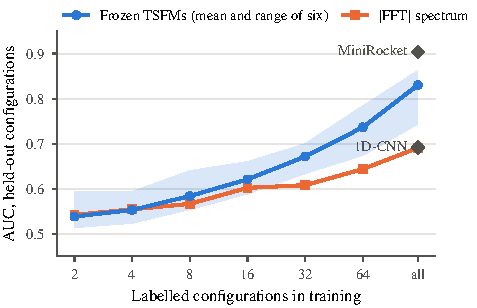
\includegraphics[width=\columnwidth]{figures/task1_label_efficiency.pdf}
  \caption{Task 1, label efficiency. AUC on held-out configurations against the number of labelled
  configurations used for training (logistic regression, sign-symmetric, mean of 5 draws and 5 folds).
  The band spans the six frozen models. Diamonds: references trained on all training configurations.}
  \label{fig:task1}
\end{figure}

On configurations not seen in training, logistic regression on frozen embeddings reaches AUC 0.83--0.86 for
five of the six models (\cref{tab:task1}). MiniRocket, which builds its features from the training folds,
does better (0.90). The 1D-CNN trained from scratch does clearly worse (0.69), as does the spectrum
baseline. TTM-R2 is the weakest frozen model (0.74).

\paragraph{Random splits leak.}
On the reference notebook's random split over all 3{,}120 signals, $k$-NN on frozen MOMENT, Mantis or TTM
embeddings reaches AUC 1.00. So does the 1D-CNN when, as in the notebook, its early-stopping data are also
drawn at random. On held-out configurations the CNN falls to 0.69, and training it for 150 instead of 40 epochs does
not help (0.62 on the first fold), so its gap is one of generalisation, not under-training.

\paragraph{Polarity is not the cue.}
A probe that only sees the sign of the largest peak is at chance (\cref{tab:task1}). Removing polarity as
a cue raises the AUC of every frozen model by 0.02 to 0.07, so the models were not exploiting it.

\paragraph{Labels help, but a few are not enough.}
Without any damage labels, Mantis still separates damaged from healthy signals on held-out configurations with AUC
0.79, using only distances to healthy training signals. With labels, \cref{fig:task1} shows that up to 8
labelled configurations are not enough for any method (AUC at most 0.64). From 32 configurations on,
every frozen model is ahead of the spectrum baseline, and the gap grows as labels are added.

\subsection{Task 2: delamination detection from healthy data only}
\label{sec:res2}

\begin{table*}[t]
  \caption{Task 2, NASA PCoE. Signal-level ROC-AUC (mean $\pm$ s.d.\ over 4 specimens $\times$ 5
  reference draws within specimen; mean over 4 held-out specimens across specimens), and the number of
  20{,}000-cycle measurements that score above every healthy test measurement of the same specimen
  (detection at zero false alarms). Best value per column in bold.}
  \label{tab:task2}
  \centering
  \small
  \begin{tabular}{@{}lcccccc@{}}
    \toprule
    & \multicolumn{4}{c}{Reference from the same specimen} &
      \multicolumn{2}{c}{Reference from the other specimens} \\
    \cmidrule(lr){2-5}\cmidrule(lr){6-7}
    Features and detector & Same-path & $k$-NN & PCA + ocSVM & Detected & Same-path & Detected \\
    \midrule
    \multicolumn{7}{@{}l}{\emph{Frozen TSFM embeddings}} \\
    \inputrows{tables/task2.tex}
    \bottomrule
  \end{tabular}
\end{table*}

\begin{figure}[t]
  \centering
  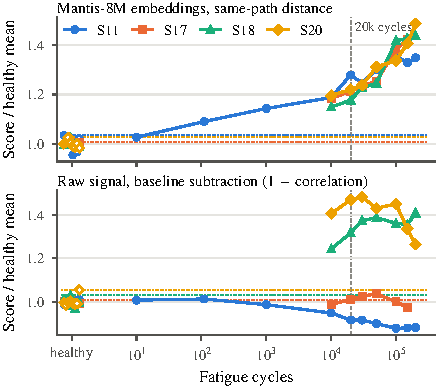
\includegraphics[width=\columnwidth]{figures/task2_cross_specimen.pdf}
  \caption{Task 2, healthy reference taken from the \emph{other} three specimens. Measurement scores of
  each specimen relative to the mean of its own healthy measurements (open markers on the left; dotted
  lines mark their maximum). With Mantis embeddings, every measurement from 10{,}000 cycles on lies above the
  specimen's healthy ones. With the best raw-signal detector, S11 falls below its healthy level and S17
  barely separates.}
  \label{fig:task2}
\end{figure}

Within a specimen, the same-path distance on frozen embeddings is as good as classical baseline
subtraction (\cref{tab:task2}): signal-level AUC 0.95--0.98 for five models (Chronos-2: 0.88), against
0.97 for $1-$correlation. With the same-path distance, every model flags all 20 damaged measurements at zero
false alarms.

\paragraph{Compare like with like.}
For every feature set the same-path distance beats the $k$-NN distance, which compares a signal with
reference signals of any path. The PCA + one-class SVM detector, pooled over all signals, is near chance
on embeddings (0.44--0.62) and below chance on raw signals (0.23): differences between paths swamp the
damage.

\paragraph{Across specimens the models separate.}
When the healthy reference comes from the other three coupons, the raw-signal detectors fall to AUC
0.15--0.57, because coupons differ from each other more than fatigue changes them. Mantis (0.81) and
Chronos-Bolt (0.67) still rank every coupon's damaged measurement above all its healthy ones, and TiRex
does so for three of the four (\cref{fig:task2}). MOMENT detects well within a specimen (0.95) but
transfers worst (0.47).

\paragraph{Damage growth.}
Within a specimen, the same-path distance keeps rising with fatigue. By 10{,}000 cycles it reaches 1.9 to
3.2 times the healthy level (geometric mean over specimens) for every model, and it keeps rising more
slowly up to 100{,}000--150{,}000 cycles (\cref{app:growth}).

\subsection{Task 3: locating damage on the plate}
\label{sec:res3}

\begin{figure*}[t]
  \centering
  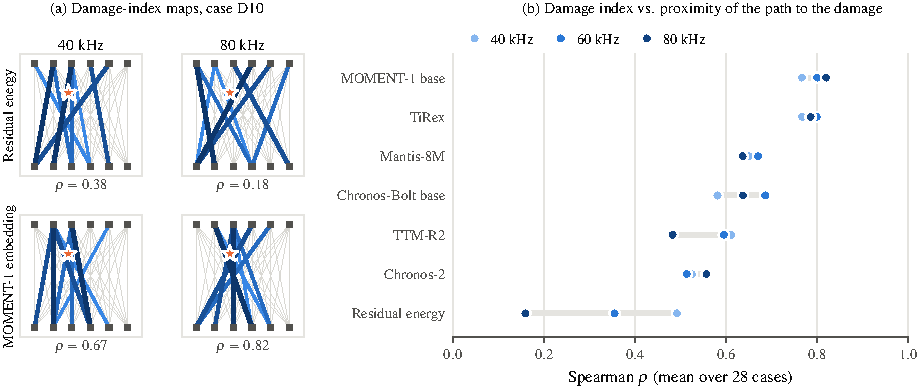
\includegraphics[width=\textwidth]{figures/task3_maps_spearman.pdf}
  \caption{Task 3, why the network view works. (a) Damage-index maps for one damage case (D10, whose
  80\,kHz correlations are close to the median for both methods). The eight paths with the highest index are drawn
  in blue, darker for higher; the star marks the damage. Residual energy is only weakly related to the damage
  position at 40\,kHz and unrelated at 80\,kHz; the MOMENT embedding distance concentrates on paths
  through the damage at both. (b) Spearman correlation between a
  path's damage index and its proximity to the damage (negative distance from the damage centre to the
  path), averaged over the 28 cases.}
  \label{fig:task3}
\end{figure*}

\begin{table}[t]
  \caption{Task 3, OGW-1, path level. Zone accuracy of single-path classification ($k$-NN for frozen
  and raw features), averaged over the three frequencies. Last column: per-path predictions averaged over
  the 36 paths of a case. Splits: random 90/10; grouped by (position, path); unseen damage positions.
  Chance is 0.14. $^\dagger$Trained on the data; run on one random split and the four unseen-position
  folds.}
  \label{tab:task3path}
  \centering
  \small
  \setlength{\tabcolsep}{3pt}
  \begin{tabular}{@{}lcccc@{}}
    \toprule
    & \multicolumn{3}{c}{One path at a time} & 36 paths \\
    \cmidrule(lr){2-4}\cmidrule(lr){5-5}
    Features & Random & Grouped & Unseen & Unseen \\
    \midrule
    \inputrows{tables/task3_path.tex}
    \bottomrule
  \end{tabular}
\end{table}

\begin{table}[t]
  \caption{Task 3, OGW-1, network level. Zone accuracy on held-out positions (28 cases per column) from
  the 36-path damage-index map with logistic regression; residual energy is the physics-based index.
  Control: healthy maps of the same phase (mean and maximum over 10 draws). Chance is 0.14.}
  \label{tab:task3net}
  \centering
  \small
  \setlength{\tabcolsep}{3pt}
  \begin{tabular}{@{}lcccccc@{}}
    \toprule
    & \multicolumn{4}{c}{Damage maps, kHz} & \multicolumn{2}{c}{Control} \\
    \cmidrule(lr){2-5}\cmidrule(lr){6-7}
    Damage index & 40 & 60 & 80 & All & Mean & Max \\
    \midrule
    \inputrows{tables/task3_network.tex}
    \bottomrule
  \end{tabular}
\end{table}

\paragraph{One path at a time, nothing works.}
Classified path by path, no method finds the zone. Accuracy in \cref{tab:task3path} stays between 0.17
and 0.29 for every feature set and split, including MiniRocket and the CNN trained on the data. The audit
in \cref{sec:data} explains why: only paths close to the damage carry a residual above the drift, so most
training examples are labelled with a zone they contain no evidence of. Averaging the per-path predictions
over the 36 paths of a case recovers part of the zone, up to 0.81 for MOMENT.

\paragraph{Read as a network, every position is found.}
The map of same-path distances solves the task (\cref{tab:task3net}). All six models place all 28 held-out
positions in the correct zone when the three frequencies are combined (95\% Clopper--Pearson interval
0.88--1.00),
and MOMENT and TiRex do so at every frequency on its own. Residual energy read by the same classifier
reaches 0.96 at 40\,kHz but drops to 0.61 at 60\,kHz and 0.25 at 80\,kHz, where the damage changes less
energy than the drift does.

\paragraph{The result is not a phase shortcut.}
With healthy maps from the same phase in place of the damage maps, accuracy falls to 0.15--0.20 on average
(chance 0.14). The phase normalisation alone does not give the zone away.



\paragraph{Why it works.}
The embedding distance of a path grows the closer the path passes to the damage, at all three
frequencies (\cref{fig:task3}). For MOMENT and TiRex the rank correlation is 0.77--0.82. Residual energy
follows proximity at 40\,kHz (0.49) and loses it at 80\,kHz (0.16), where drift dominates the energy.

\paragraph{The classifier is still needed.}
In training-free RAPID tomography the embedding distances localise worse than residual energy at 40\,kHz
(0.32--0.50 against 0.75) and better at 80\,kHz (0.29--0.61 against 0.07; \cref{app:rapid}). Their contrast
is not proportional to proximity in the way RAPID assumes, but the pattern over paths is consistent enough
for a linear classifier to read.

% ---------------------------------------------------------------------------------------------
\section{Discussion}
\label{sec:discussion}

\paragraph{What transfers.}
A distance between embeddings of the same path behaves like a learned, nonlinear baseline subtraction. It
is as sensitive as classical subtraction within a specimen, and less disturbed by the variations that break
raw subtraction: differences between coupons in Task 2 and drift between baseline and damage sessions in
Task 3. What does not transfer is the idea that one signal, on its own, says where the damage is. That
fails for frozen and trained models alike, because the information is spread over the network.

\paragraph{No model wins everywhere.}
MOMENT and TiRex are best when labels are available (Task 1) and their distances track the damage most
closely (Task 3). Mantis, the only model pretrained for classification, is best without labels, both on
Task 1 and across specimens in Task 2. TTM-R2, the smallest model, is weakest in most settings, but size is
not decisive otherwise: Mantis has 8M parameters and Chronos-Bolt 205M. A practitioner should therefore
try several models, and should validate across specimens, not only within one.

\paragraph{Evaluation pitfalls.}
\label{sec:pitfalls}
Four choices change the conclusions on these datasets. Random splits over repeated acquisitions score AUC
1.00 for almost any method (Task 1). Sign-inverted signals could stand in for damage; a polarity probe and
sign-symmetric training rule this out (Task 1). Normalising each damage case by the baselines of its own
measurement phase opens a possible shortcut, which a healthy-map control rules out (Task 3). Finally,
per-path zone labels are ill-posed for paths far from the damage, so localisation should be scored on the
network (Task 3).

\paragraph{Limitations.}
The number of independent units is small: 156 sensor configurations, four specimens and 28 damage
positions, so confidence intervals are wide. In the NASA data we use one boundary condition and, as in
earlier work, label the 20{,}000-cycle state as damaged without an independent damage measurement. OGW-1
was recorded at constant temperature, so environmental variation is not tested in Tasks 2 and 3. The
embeddings are mean-pooled and never fine-tuned, and other TSFMs such as TimesFM and Moirai were not
tested. In exploratory work we also used the models as forecasters along the temperature axis of another
OGW dataset; physics-based compensation was far more accurate, so we did not pursue forecasting as a
monitoring framing.

% ---------------------------------------------------------------------------------------------
\section{Conclusion}
\label{sec:conclusion}

Frozen time series foundation models, never trained on ultrasonic data, carry enough information about
guided waves to detect, classify and locate damage in composite structures. The condition is to use them
the way the field has always used signals: compare each one with healthy recordings of its own sensor
path, and read the network of paths together. Under that condition, a pretrained model with a linear
head matches classical damage indices, transfers better across specimens, beats a CNN trained from
scratch and comes close to MiniRocket, all without fine-tuning and on a CPU. Testing the same recipe under changing temperature and on larger
structures is the natural next step.

% ---------------------------------------------------------------------------------------------
\section*{Software and Data}
All three datasets are public. \ificmlshowauthors Code, result tables and download scripts are available at
\url{https://github.com/mahindrautela/gwshm-tsfm}.\else Code, result tables and download scripts are
provided as supplementary material and will be released publicly.\fi{} Every experiment runs on a two-core
CPU in one Python environment.

\section*{Impact Statement}
This work concerns monitoring of safety-critical structures. The methods are research results on small
laboratory datasets and are not a substitute for certified inspection. A missed detection in practice can
have serious consequences, so any deployment would need validation on the target structure, under its
operating conditions, with false-alarm and missed-detection rates set by the relevant certification
process. We see no other societal consequences that need to be highlighted here.

\bibliography{references}
\bibliographystyle{icml2026}

% ---------------------------------------------------------------------------------------------
\newpage
\appendix
\onecolumn

\section{Dataset Details}
\label{app:data}

\paragraph{GW-TCW.} The baseline and damage files each hold 1{,}560 signals of 1{,}000 samples at 2\,MHz
(0.5\,ms). Row $i$ belongs to configuration $(\lfloor i/120\rfloor, i \bmod 12)$: 13 blocks of 120 rows,
each holding 10 repeated acquisitions of 12 sensor paths, and baseline row $i$ and damaged row $i$ share
a configuration. The median correlation between repeats of a configuration is 0.99997 (minimum 0.9994).
We keep the first acquisition of each configuration. The leaky split of the reference notebook uses all
3{,}120 signals with a random 95/5 split.

\paragraph{NASA PCoE.} Each measurement holds 252 signals: actuators 1--6 to sensors 7--12 (36 paths) at
150, 200, \dots, 450\,kHz. Healthy measurements are those at 0--3 cycles, 8 per specimen. Damage-growth
measurements are taken at 10, 110, 1{,}000, 10{,}000, 20{,}000, 30{,}000, 50{,}000, 100{,}000, 150{,}000 and
200{,}000 cycles where available, the first repetition at each count (30 in total; only S11 has the counts
below 10{,}000).

\paragraph{OGW-1.} Signals are recorded at 10\,MHz with 13{,}108 samples and decimated to 1\,MHz. The
excitation onset is read from the recorded excitation signal. Transducers T1--T6 sit at $y=470$\,mm and
T7--T12 at $y=30$\,mm, at $x=450, 370, \dots, 50$\,mm; the 36 crossing paths are T$i$--T$j$ with
$i\le 6<j$. The 28 defect positions form seven $2\times2$ clusters with 15\,mm spacing. Distances in the
audit and in \cref{fig:task3} are from the defect centre to the transmitter--receiver segment.

\begin{table}[H]
  \caption{OGW-1 audit: median residual energy of a path relative to the baseline-to-baseline drift of the
  same path and phase, by distance between path and damage (48 near and 448 far path--case pairs per
  frequency).}
  \label{tab:audit}
  \centering
  \small
  \begin{tabular}{@{}lccc@{}}
    \toprule
    Paths & 40\,kHz & 60\,kHz & 80\,kHz \\
    \midrule
    within 10\,mm of the damage & 4.24 & 2.36 & 0.81 \\
    more than 120\,mm away & 0.71 & 0.67 & 0.60 \\
    \bottomrule
  \end{tabular}
\end{table}

\section{Implementation Details}
\label{app:impl}

\paragraph{Embeddings.} \Cref{tab:checkpoints} lists the checkpoints and how each signal is turned into
one vector. TTM-R2 uses a context of 1{,}024. NASA and OGW-1 embeddings are stored in half precision.

\begin{table}[H]
  \caption{Checkpoints and pooling.}
  \label{tab:checkpoints}
  \centering
  \small
  \begin{tabular}{@{}lll@{}}
    \toprule
    Model & Checkpoint & Embedding of one signal \\
    \midrule
    Chronos-2 & \texttt{amazon/chronos-2} & mean over the encoder's patch tokens \\
    Chronos-Bolt base & \texttt{amazon/chronos-bolt-base} & mean over the encoder's patch tokens \\
    TiRex & \texttt{NX-AI/TiRex} & output of the package's embedding module \\
    MOMENT-1 base & \texttt{AutonLab/MOMENT-1-base} & embedding task head (mean of patch embeddings) \\
    Mantis-8M & \texttt{paris-noah/Mantis-8M} & the trainer's \texttt{transform} \\
    TTM-R2 & \texttt{ibm-granite/granite-timeseries-ttm-r2} & mean over patches of the backbone hidden state \\
    \bottomrule
  \end{tabular}
\end{table}

\paragraph{Heads.} Features are standardised with training statistics. Logistic regression uses L2
regularisation with $C=1$ (Tasks 1 and 3, path level) or $C=0.1$ (Task 3, network level, 21 training cases
with 36 to 108 features). $k$-NN uses $k=5$ and cosine distance. The $k$-NN anomaly score in Task 2 is the
Euclidean distance to the nearest standardised reference signal. The one-class SVM uses an RBF kernel and
$\nu=0.1$ on 10 principal components.

\paragraph{Trained references.} MiniRocket uses its default settings, followed by a ridge classifier
whose penalty is chosen by internal cross-validation. The 1D-CNN follows the GW-TCW reference notebook:
four convolution layers with 16, 32, 64 and 128 filters, Adam with learning rate $10^{-3}$, 40 epochs and
early stopping on held-out training configurations. In Task 3 the CNN uses early stopping on held-out
groups.

\paragraph{RAPID.} Each path contributes $\max(\mathrm{DI}_p-1,0)$ inside an ellipse with foci at its
transducers ($\beta=1.05$) on a 5\,mm grid; the predicted zone is the one whose centre is nearest the
image maximum.

\section{Additional Results}
\label{app:results}

\subsection{Damage growth (Task 2)}
\label{app:growth}

\begin{table}[H]
  \caption{Same-path distance of later measurements relative to the healthy level, within specimen
  (geometric mean over specimens of the ratio to the mean healthy test score; 200k: three specimens).}
  \label{tab:growth}
  \centering
  \small
  \begin{tabular}{@{}lccccccc@{}}
    \toprule
    Features & 10k & 20k & 30k & 50k & 100k & 150k & 200k \\
    \midrule
    \inputrows{tables/task2_growth.tex}
    \bottomrule
  \end{tabular}
\end{table}

\subsection{Training-free localisation with RAPID (Task 3)}
\label{app:rapid}

\begin{table}[H]
  \caption{RAPID tomography on the damage-index maps: zone accuracy (median localisation error in mm).}
  \label{tab:rapid}
  \centering
  \small
  \begin{tabular}{@{}lccc@{}}
    \toprule
    Damage index & 40\,kHz & 60\,kHz & 80\,kHz \\
    \midrule
    \inputrows{tables/task3_rapid.tex}
    \bottomrule
  \end{tabular}
\end{table}

\subsection{Path-level localisation with logistic regression (Task 3)}

\begin{table}[H]
  \caption{As \cref{tab:task3path}, with logistic regression instead of $k$-NN.}
  \label{tab:task3pathlr}
  \centering
  \small
  \begin{tabular}{@{}lcccc@{}}
    \toprule
    & \multicolumn{3}{c}{One path at a time} & 36 paths \\
    \cmidrule(lr){2-4}\cmidrule(lr){5-5}
    Features & Random & Grouped & Unseen & Unseen \\
    \midrule
    \inputrows{tables/task3_path_lr.tex}
    \bottomrule
  \end{tabular}
\end{table}

% ---------------------------------------------------------------------------------------------
\section{Extended Experiments}
\label{app:ext}

The experiments in this appendix were run after the main study. They leave the protocols, splits and
results of Tasks 1--3 unchanged and are produced by separate scripts (\texttt{scripts/ext\_*.py}); every
table below is generated from their outputs. Extended embeddings were computed on an Apple GPU
(\texttt{mps}); for the six paper models this changes Task~2 AUCs by at most $10^{-4}$, except for Mantis,
whose embeddings are wrong on that backend and which therefore stays on the CPU.

\subsection{Temperature (OGW CFRP temperature dataset)}
\label{app:ext:temp}

\paragraph{Protocol.} The plate of OGW-1 was also measured in a climate chamber stepped from 20 to
60\,\textdegree C and back in 0.5\,\textdegree C steps \citep{moll2019ogw}: two cycles without damage and
one cycle each with the reversible defect at D4, D12, D16 or D24 (161 measurements per cycle, 40\,kHz, the
36 crossing paths, 1{,}024 samples at 1\,MHz). Healthy references are taken from the first undamaged
cycle on a temperature grid with spacing $s$ (for each grid point, the nearest measurement of the heating
and of the cooling half); the second undamaged cycle is the healthy test and the four damaged cycles are
the damaged test. A measurement's score is the mean over its paths of a per-path index: the same-path
embedding distance (\cref{eq:samepath}) to the mean reference, to the reference at the nearest
temperature (NT) or to the closest reference (OBS, optimal baseline selection in embedding space); and,
on raw signals, the residual energy against the NT reference, against the best reference (OBS), against
the NT reference stretched in time by the best factor in 0.96--1.04 (BSS, baseline signal stretch), or
both (OBS + BSS, over the three nearest references). Thresholds for a nominal false-alarm rate are the
quantiles of leave-one-out scores of the first cycle, so no test data are used.

\begin{table}[H]
  \caption{Temperature robustness. ROC-AUC (healthy second cycle vs damaged cycles) as a function of the
  spacing of the reference temperatures, and detection rate at a nominal 5\% false-alarm rate (realised
  rate on the healthy test in brackets) for spacings of 2 and 5\,\textdegree C. Embedding rows: the three
  models with the highest OBS AUC averaged over spacings; all nine are in \texttt{results/ext\_temperature}.}
  \label{tab:ext:temp}
  \centering
  \small
  \begin{tabular}{@{}lcccccccc@{}}
    \toprule
    & \multicolumn{6}{c}{AUC, reference spacing (\textdegree C)} & \multicolumn{2}{c}{Detected at 5\%} \\
    \cmidrule(lr){2-7}\cmidrule(lr){8-9}
    Detector & 0.5 & 2 & 5 & 10 & 20 & 40 & 2\,\textdegree C & 5\,\textdegree C \\
    \midrule
    \inputrows{tables/ext_temperature.tex}
    \bottomrule
  \end{tabular}
\end{table}

\paragraph{Results.} With references every 0.5--2\,\textdegree C, the closest-reference embedding
distance is as good as classical compensation (AUC 0.98--1.00 for TiRex, MOMENT and both Chronos
models; raw OBS + BSS 1.00). As the references thin out, classical compensation degrades more slowly: at
5\,\textdegree C spacing OBS + BSS reaches 0.98 and BSS alone 0.89, against 0.92 for the best embedding
(TiRex); at 10\,\textdegree C, 0.87 against at most 0.74; from 20\,\textdegree C on every method is near
chance. Without temperature handling, the mean-reference distance that works in Task~2 fails here
(0.49--0.69): temperature changes a path more than the defect does. At a fixed false-alarm rate the
embeddings fall further behind: with references every 5\,\textdegree C, OBS + BSS detects 73\% of the
damaged measurements at a realised 1\% false-alarm rate; the best embedding detects 17\% (Mantis, nearest
temperature, at a realised 8\%).

\paragraph{Controls.} Damage is confounded with recording time (the sessions span one month). A trigger
offset between sessions would be a shortcut; the median lag of every session against the first cycle is
below 0.1 sample. A drift between the two healthy cycles would raise healthy test scores; it does not
(healthy test vs leave-one-out first-cycle scores: AUC at most 0.53). Finally, paths closer to the defect
change more than distant ones (Spearman 0.56--0.64 for the raw detectors, 0.3--0.6 for most embeddings
with OBS; weak for Chronos and Mantis), so the detections are at least partly local to the damage.

\subsection{More models and pooling}
\label{app:ext:models}

\paragraph{Models.} TimesFM~2.5 (231M parameters, \texttt{google/timesfm-2.5-200m-pytorch}), Sundial base
(128M, \texttt{thuml/sundial-base-128m}) and Moirai~2.0-R small (11M, \texttt{Salesforce/moirai-2.0-R-small})
are added through the same interface: each signal is prepared as the model's own forecasting code
prepares its context, and the decoder's patch tokens are averaged. \Cref{tab:ext:models} runs the
unchanged Task 1--3 protocols on all nine models; the six paper models reproduce the main tables exactly in
this run. Sundial ties the best models on Task~1 and, with Moirai~2, transfers best across NASA coupons
(AUC 0.83--0.84, all four coupons detected). TimesFM~2.5 is weak on Task~1 (0.75) but locates every
damage position.

\begin{table}[H]
  \caption{Nine frozen models under the paper's protocols. T1: GW-TCW, sign-symmetric logistic
  regression AUC. T2: NASA, same-path distance, signal AUC within and across specimens, and coupons
  detected at zero false alarms across specimens. T3: OGW-1 network level, zone accuracy (mean of 40, 60,
  80\,kHz; three frequencies combined) and Spearman correlation of the DI with path proximity (mean over
  frequencies). $^\star$Added in this appendix.}
  \label{tab:ext:models}
  \centering
  \small
  \begin{tabular}{@{}lccccccc@{}}
    \toprule
    & T1 & \multicolumn{3}{c}{T2} & \multicolumn{3}{c}{T3} \\
    \cmidrule(lr){2-2}\cmidrule(lr){3-5}\cmidrule(lr){6-8}
    Model & AUC & Within & Across & Det. & Acc. (per freq.) & Acc. (all) & $\rho$ \\
    \midrule
    \inputrows{tables/ext_models.tex}
    \bottomrule
  \end{tabular}
\end{table}

\paragraph{Pooling.} Forward hooks record every block of each model in the same pass, and seven
read-outs are scored with the same protocols (\cref{tab:ext:pooling}). The last token, the natural summary
of the causal models, is the worst read-out on average and loses most of the localisation signal
($\rho$ 0.42). Intermediate blocks are often better than the final one: the block at half depth improves
cross-specimen detection for seven of nine models and the Spearman correlation for six. The best single
read-outs (Sundial at half depth, Task~1 AUC 0.89; Chronos-2 at a quarter depth, Task~2 within-specimen
0.98 instead of 0.88) were found by looking at the test protocols, so they indicate headroom rather than
an unbiased estimate.

\begin{table}[H]
  \caption{Pooling ablation: mean over the nine models of each task's headline metric (as in
  \cref{tab:ext:models}; T3 accuracy is the mean over the three single frequencies), and in brackets the
  number of models for which the read-out beats the model's own embedding.}
  \label{tab:ext:pooling}
  \centering
  \small
  \begin{tabular}{@{}lccccc@{}}
    \toprule
    Read-out & T1 AUC & T2 within & T2 across & T3 acc. & T3 $\rho$ \\
    \midrule
    \inputrows{tables/ext_pooling.tex}
    \bottomrule
  \end{tabular}
\end{table}

\subsection{Other NASA layups and boundary conditions}
\label{app:ext:nasa}

\paragraph{Protocol.} The NASA data also contain layups 1 and 3 and two further boundary conditions,
clamped and traction-free, with fewer early-life repeats (2--7 per specimen) and a 20{,}000-cycle
measurement for only some specimens. The Task~2 selection is applied unchanged to every combination
(layup~2, loaded, reproduces the paper's array exactly). Within a specimen, half of its healthy
measurements form the reference (every split if there are at most five, else five random ones); across
specimens, the other coupons of the same layup and condition; across layups, every healthy measurement of
another layup under the loaded condition. Signals are scaled by healthy data only.

\begin{table}[H]
  \caption{Same-path distance on all layups and boundary conditions: signal AUC, mean over specimens
  (specimens whose 20k measurement scores above all their healthy test measurements / specimens with a
  20k measurement). Cross-specimen and cross-layup: loaded condition.}
  \label{tab:ext:nasa}
  \centering
  \small
  \begin{tabular}{@{}llccccc@{}}
    \toprule
    & & \multicolumn{3}{c}{Within specimen} & Across & Across \\
    \cmidrule(lr){3-5}
    Layup & Features & Loaded & Clamped & Traction free & specimens & layups \\
    \midrule
    \inputrows{tables/ext_nasa.tex}
    \bottomrule
  \end{tabular}
\end{table}

\paragraph{Results.} Within a specimen, the result of Task~2 generalises to every layup and boundary
condition: AUC 0.82--1.00 under load and 0.70--0.99 clamped or traction-free, with the 20{,}000-cycle
measurement detected at zero false alarms in 215 of 216 model--specimen cases. Across specimens, transfer
holds under load for all three layups (Sundial, Moirai~2 and Mantis 0.79--0.86, every damaged coupon
detected; raw-signal detectors 0.15--0.57), but not for the clamped and traction-free conditions (embeddings
0.36--0.74). These two unloaded conditions give almost identical signals (median correlation 0.95--0.98
for the same specimen and cycle count, against 0.38--0.69 with the loaded condition). A healthy reference
from another layup works partly: 0.66--0.80 for Moirai~2, which detects every damaged coupon, against
0.44--0.48 for raw $1-$correlation.

\subsection{Uncertainty and significance}
\label{app:ext:stats}

\paragraph{Protocol.} Intervals resample the physical unit of each task. Task~1: out-of-fold scores on the
paper's folds, AUC with a 95\% bootstrap interval over the 156 configurations, paired bootstrap tests
between methods with Holm correction, and the whole cross-validation repeated with 20 fold assignments.
Task~2: all $\binom{8}{4}=70$ reference splits per specimen; with four specimens, an exact paired test
cannot reach $p<0.125$. Task~3: per-position correctness with Clopper--Pearson intervals and exact McNemar
tests.

\begin{table}[H]
  \caption{Uncertainty over physical units. T1: pooled out-of-fold AUC [95\% bootstrap interval over
  configurations] and mean $\pm$ s.d.\ over 20 fold assignments. T2: within-specimen same-path AUC over all
  70 reference splits (worst split) and share of splits detected at zero false alarms. T3: positions
  located from the three-frequency map [Clopper--Pearson 95\%].}
  \label{tab:ext:stats}
  \centering
  \small
  \begin{tabular}{@{}lccccc@{}}
    \toprule
    & \multicolumn{2}{c}{T1} & \multicolumn{2}{c}{T2} & T3 \\
    \cmidrule(lr){2-3}\cmidrule(lr){4-5}\cmidrule(lr){6-6}
    Features & AUC [CI] & 20 fold sets & AUC (worst) & Detected & Correct [CI] \\
    \midrule
    \inputrows{tables/ext_stats.tex}
    \bottomrule
  \end{tabular}
\end{table}

\paragraph{Which differences are significant.} In Task~1 the seven strongest frozen models (MOMENT,
TiRex, Sundial, Chronos-Bolt, Chronos-2, Moirai, Mantis) cannot be separated: every pairwise difference is
at most 0.04 AUC with uncorrected $p\ge0.11$, and the choice of folds alone moves a model by about 0.02.
TTM-R2 and TimesFM~2.5 are significantly below MOMENT, TiRex, Sundial and Chronos-Bolt, and the seven
strongest frozen models are significantly above the \fft{} baseline (Holm-corrected $p<0.05$). MiniRocket's advantage is significant against Mantis
and Moirai but, after correction, not against MOMENT, TiRex, Sundial or the Chronos models (uncorrected
$p$ = 0.01--0.08). In Task~2 no difference in \cref{tab:task2} can be significant at the level of
specimens; every model still detects the damaged state in all 280 within-specimen runs. In Task~3, with the
three frequencies combined, 28/28 against 25/28 for residual energy is not significant ($p=0.25$); at
80\,kHz every embedding is significantly better than residual energy (Holm-corrected $p\le0.04$).

\subsection{Coordinates, unseen zones and missing sensors (Task 3)}
\label{app:ext:task3}

\paragraph{Protocol.} From the same log-DI maps: ridge regression of the defect centre in mm under the
paper's leave-position-out folds; a leave-one-zone-out split, where the four positions of a zone are never
seen in training (only regression can be scored), with the healthy-map control; and missing sensors at
test time (1--4 transducers or 10--50\% of the paths, 20 random draws), with the classifier retrained on
the remaining paths.

\begin{table}[H]
  \caption{Task 3 beyond seven zones. Median localisation error (mm) of ridge regression on the
  three-frequency map (leave position out), of RAPID at 40\,kHz, and of ridge regression with a whole zone
  held out (healthy-map control alongside; predicting the mean training position gives 174\,mm). Last
  columns: zone accuracy with 2 or 4 transducers, or half of the paths, missing.}
  \label{tab:ext:task3}
  \centering
  \small
  \begin{tabular}{@{}lccccccc@{}}
    \toprule
    & \multicolumn{2}{c}{Seen zones} & \multicolumn{2}{c}{Unseen zone} & \multicolumn{3}{c}{Missing} \\
    \cmidrule(lr){2-3}\cmidrule(lr){4-5}\cmidrule(lr){6-8}
    Damage index & Ridge & RAPID & Ridge & Control & 2 T & 4 T & 50\% \\
    \midrule
    \inputrows{tables/ext_task3.tex}
    \bottomrule
  \end{tabular}
\end{table}

\paragraph{Results.} Regressing coordinates locates the defect to a median of 22\,mm (MOMENT) to 72\,mm,
against 66\,mm for residual energy and 72--126\,mm for RAPID; with the zone known, the zone centre is
11\,mm from the defect, so regression is less precise than the seven-zone classifier on known zones and
mainly useful as a continuous estimate. Extrapolation to a zone never seen in training largely fails:
errors of 119--225\,mm against 174--187\,mm without any damage information. Only the zone in the middle of
the plate (D9--D12) is found by every method (16--86\,mm); the zones at the plate edges are not. Missing sensors cost little: with four of twelve transducers lost, TiRex, MOMENT,
TimesFM~2.5 and Sundial still locate 99--100\% of the positions after retraining, residual energy 70\%.

\subsection{Light adaptation}
\label{app:ext:adapt}

\paragraph{Protocol.} MOMENT and TiRex, the strongest Task~1 models, are adapted on the GPU under the
Task~1 folds and sign symmetry. The head starts from the paper's logistic regression on the frozen
features; 20\% of the training configurations are held out for early stopping, and the starting point
itself is kept if no epoch improves the validation AUC. Variants: the linear head alone, the last two blocks
unfrozen, or rank-8 LoRA adapters in the last six blocks (MOMENT: attention; TiRex: feed-forward
projections). TiRex pads every input to its 2{,}048-sample context with NaN, which makes the gradients of
its first blocks undefined; only its last six blocks, whose gradients are finite, are trained. The TiRex
feature here is the last block's mean (0.80 with the paper's head), not the package's all-layer embedding.

\begin{table}[H]
  \caption{Light adaptation, Task 1 (AUC, mean $\pm$ s.d.\ over the five folds).}
  \label{tab:ext:adapt}
  \centering
  \small
  \begin{tabular}{@{}lcccc@{}}
    \toprule
    Model & Linear probe (paper head) & Linear head (gradient) & Last 2 blocks & LoRA $r=8$ \\
    \midrule
    \inputrows{tables/ext_adapt.tex}
    \bottomrule
  \end{tabular}
\end{table}

\paragraph{Results.} EXT-ADAPT-RESULTS

\end{document}
